% 20/5/11 Jan verbetert enkele foutjes en past twee laatste progs aan 
% 14/12/10 Greetje wijzigt om geheel beter te structureren
% 15/09/10 Greetje werkt voorbeelden verder uit en ook al de rest
% 7/12/09 Jan verandert variaties naar permutaties
% 8/12/09 Greetje verandert ook nog wat kleinigheden




%\lstset{language=Scilab,basicstyle=\ttfamily \footnotesize,backgroundcolor=\color{white},
frame=single,framerule=0.5pt,numbers=left,tabsize=2}
%\lstdefinestyle{inline} {basicstyle=\normalsize \ttfamily}


\chapter{Algoritmes en Telproblemen}

\vbsection{Algoritmes}

\subsection{Inleiding}

Een algoritme is een stappenplan waarmee je een probleem kan oplossen. In het kader van de opleiding Toegepaste informatica zien we algoritmes als een rij instructies voor een computer zodat die weet wat hij moet doen. Het spreekt voor zich dat in dat laatste geval elke stap heel precies omschreven moet worden.

Een algoritme is een eindige verzameling instructies met volgende kenmerken:
\begin{itemize}
\item precisie: elke stap is heel precies omschreven;
\item uniciteit: tussenliggende resultaten zijn altijd uniek gedefinieerd en hangen alleen af van de input en de resultaten van de tussenliggende stappen;
\item eindigheid: het algoritme stopt na een eindig aantal stappen;
\item input: het algoritme vertrekt van een beginsituatie;
\item output: het algoritme heeft een resultaat;
\item algemeenheid: het algoritme werkt bij verschillende soorten invoer.
\end{itemize}

Listing~\ref{lst:max} toont een algoritme dat het maximum bepaalt van drie getallen \lstinline{a}, \lstinline{b} en \lstinline{c}. Dit algoritme voldoet aan de hierboven beschreven kenmerken. De werking van het algoritme leer je begrijpen door simulatie: stel bijvoorbeeld \lstinline{a=1}, \lstinline{b=5} en \lstinline{c=3}. Welke waarden neemt \lstinline{y} achtereenvolgens aan?

\begin{lstlisting}[caption={Vind het maximum van drie getallen \lstinline{a}, \lstinline{b} en \lstinline{c}}, label={lst:max}]
  y=a;
  
  if (b>y)
    y=b;
  end
  
  if (c>y)
    y=c;
  end
\end{lstlisting}

\subsection{Complexiteit van een algoritme}

Een algoritme is soms bij een bepaalde input niet uitvoerbaar omwille van te grote uitvoeringstijd of omwille van problemen met de opslagcapaciteit van de machine.  Met  ``complexiteit van een algoritme'' verwijzen we naar de  \emph{benodigde hoeveelheid tijd  en ruimte} om het algoritme uit te voeren. In hetgeen volgt beperken we ons tot de benodigde hoeveelheid tijd.

Bekijk bijvoorbeeld volgend probleem. Gegeven de verzameling $X$ met $n$ elementen die rood of zwart kunnen zijn. Hoeveel deelverzamelingen met minstens één rood element heeft $X$? Je kan dit probleem oplossen door alle deelverzamelingen van $X$ uit te proberen. Men kan aantonen dat het aantal deelverzamelingen van de verzameling $X$ gelijk is aan $2^n$. Als je dus alle deelverzamelingen van $X$ zou uitproberen, zou je $2^n$ tijdseenheden nodig hebben. In het hoofdstuk ``Exponentiële groei'' heb je geleerd dat $2^n$ ontzettend snel groeit als $n$ wat groter is. De uitvoeringstijd van bovenstaand probleem wordt dus snel groot als het aantal elementen van $X$ toeneemt.

Het is niet eenvoudig om de uitvoeringstijd van een programma exact te bepalen. De  omvang én aard van de  input spelen een belangrijke rol, evenals de snelheid van de computer, de manier waarop het programma wordt omgezet naar machine-instructies enz. Omdat we niet al deze kenmerken 
in rekening kunnen brengen, bekijken we enkel de complexiteit van de uitvoeringstijd van het algoritme.

De uitvoeringstijd hangt af van de input.  Het exacte verband tussen de uitvoeringstijd en de input ($n$) is erg moeilijk te bepalen. Daarom bestudeert men meestal het verband tussen de uitvoeringstijd en de \emph{omvang} van de input. 

Om de uitvoeringstijd exact te bepalen zou je het aantal instructies dat uitgevoerd wordt moeten tellen. Bij een meer ruwe schatting kan je het aantal keer dat een lus doorlopen wordt tellen, of het aantal vergelijkingen dat gemaakt wordt.

Meestal zijn we niet geïnteresseerd in de exacte best-case time of worst-case time, maar wel op welke manier die veranderen als de grootte van de input ($n$) verandert. We noemen dit de \emph{orde} van de uitvoeringstijd.

\subsection{Orde van een functie}
Als we de orde van een functie bepalen, vergelijken we het verloop van die functie met een aantal standaardfuncties. Enkele van die standaardfuncties vind je in figuur~\ref{fig:standaardfuncties}. Als je tot het besluit komt dat een eerste functie zich gedraagt zoals de functie $f(n)=n^2$ en een tweede functie zoals $g(n)=2^n$, weet je dat de tweede functie veel sneller groeit dan de eerste. In deze sectie tonen we op een intiuïtieve manier het verband tussen een functie en zijn orde aan.



\begin{figure}[htbp]
\begin{center}
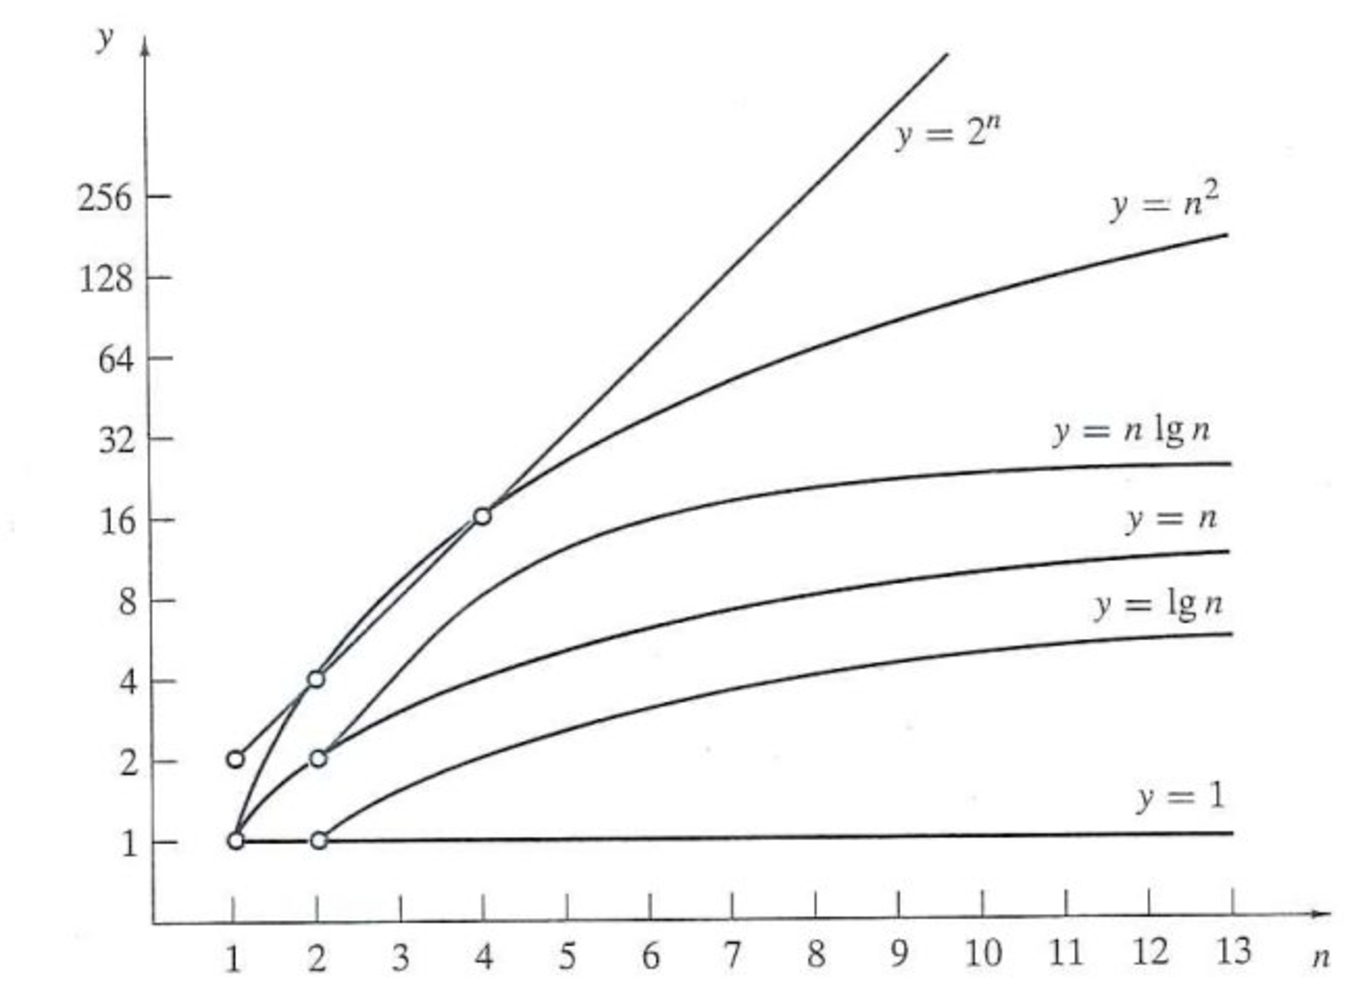
\includegraphics[width=0.7\textwidth]{figuren/telproblemen/functies.pdf}
\caption{Enkele functies. Bron: Discrete Mathematics, R. Johnsonbaugh}
\label{fig:standaardfuncties}
\end{center}
\end{figure}





We nemen als voorbeeld de functie 
\begin{equation}
	t(n)=60n^2+5n+1
	\label{eq:nkwad}
\end{equation}
Als $n$ voldoende groot is, is de functie $t(n)$ ongeveer gelijk aan $60n^2$.  Dit wordt geïllustreerd in tabel~\ref{table:nkwad}. We zeggen dat $t(n)$ \emph{groeit} zoals $60n^2$. 
\begin{table}[h]
\caption{Vergelijking van de groei van $t(n)$ met $60n^2$}
\label{table:nkwad}
\centering
\begin{tabular}{rrr}
\toprule
$n$&$t(n)=60n^2+5n+1$&$60n^2$ \\
\midrule
10&6.051&6.000\\
100&600.501&600.000\\
1.000&60.005.001&60.000.000\\
10.000&6.000.050.001&6.000.000.000\\
\bottomrule
\end{tabular}
\end{table}

Stel dat vergelijking~\eqref{eq:nkwad} de uitvoeringstijd meet in seconden, dan meet 
\begin{equation*}
T(n)=n^2+\frac5{60}n+\frac1{60}
\end{equation*}
de uitvoeringstijd in minuten. Merk op dat de coëfficiënten in de functie veranderen, maar de grootte-orde niet. De coëfficiënten zeggen niets over de grootte van de tijd, maar alleen iets over de tijds\emph{eenheid}. We zoeken daarom niet alleen de dominante term ($60n^2$ in bovenstaand voorbeeld), maar we laten ook de coëfficiënten weg. We zeggen dan ook dat $t(n)$ een functie is \emph{van orde} $n^2$. We noteren dit als
\begin{equation*}
t(n)=\Theta(n^2)\,.
\end{equation*}

In wat volgt bespreken we een systematische manier om de orde van een functie te bepalen.

\subsection{Definities}
Veronderstel de functies $f$ en $g$ met domein $\{1,~2,~3,~\dots\}$.
We schrijven
\[
f(n)=O(g(n))
\]
en zeggen dat $f(n)$ \emph{is ten hoogste van orde} $g(n)$ als er een positieve constante $C_1$ bestaat zodat
\[
|f(n)|\leq C_1|g(n)|
\]
voor alle  positieve gehele getallen $n$, op een eindig aantal uitzonderingen na. Men noemt dit soms de `grote O'-notatie.

We schrijven
\[
f(n)=\Omega(g(n))
\]
en zeggen dat $f(n)$ \emph{is ten minste van orde} $g(n)$ als er een positieve constante $C_2$ bestaat zodat
\[
|f(n)|\geq C_2|g(n)|
\]
voor alle  positieve gehele getallen $n$, op een eindig aantal uitzonderingen na.  Men spreekt over de `omega'-notatie.

We schrijven
\[
f(n)=\Theta(g(n))
\]
en zeggen dat $f(n)$ \emph{is van orde} $g(n)$ als $f(n)=O(g(n))$ en $f(n)=\Omega(g(n))$. Dit lees je als `theta'-notatie.

Als $f(n)=O(g(n))$ wil dat zeggen dat de functie $f$ niet sneller groeit dan de functie $g$. Je kan een constante zoeken ($C_1$). Als je de absolute waarde van de  functie $g$ vermenigvuldigt met die constante, zal de grafiek van die nieuwe functie altijd \emph{boven} de grafiek van de absolute waarde van $f$ liggen. Dit wordt geïllustreerd in voorbeeld~\thesection.\ref{vb:1} en figuur~\ref{fig:vb21}.

\subsection{Voorbeelden}

\voorbeeld

We bepalen de orde van 
\[
f(n)=2n+3\log n
\]

Om de orde van een functie te bepalen, gaan we in twee stappen te werk: eerst zoeken we een bovengrens voor de functie, daarna een benedengrens.

De functie $g(n)$ is een bovengrens van de functie $f(n)$ als $f(n)\leq g(n)$ voor bijna alle waarden van $n$. Omdat we gefocust zijn op de orde van $f$, proberen we de functie $f$ zo af te schatten dat $g$ een scalair veelvoud van één van de standaardfuncties is.

Omdat $\log n<n$  als $n\geq1$, is 
\[2n+3\log n <2n+3n=5n\,.\] 


zodat 
\[2n+3\log n=O(n)\] 

Omdat  $\log n\geq0$ als $n\geq1$, is 
\[2n+3\log n \geq 2n\] 
zodat
\[2n+3\log n =\Omega(n)\,.\] 

Hieruit besluiten we
\[2n+3\log n =\Theta(n)\,.\]

\voorbeeld
\label{vb:1}
Als $n>1$, dan is
\[
60n^2+5n+1\leq60n^2+5n^2+n^2=66n^2\,.
\]
Kies $C_1=66$ en $g(n)=n^2$. Dan is 
\[
|60n^2+5n+1|\leq C_1|g(n)|
\]
zodat 
\[60n^2+5n+1=O(n^2)\,.
\] 

Als $n>1$, dan is
\[
60n^2+5n+1\geq60n^2\,.
\]
Kies $C_2=60$ en $g(n)=n^2$. Dan is 
\[
|60n^2+5n+1|\geq C_2|g(n)|
\]
zodat 
\[60n^2+5n+1=\Omega(n^2)\,.
\] 

Omdat $60n^2+5n+1=O(n^2)$ en $60n^2+5n+1=\Omega(n^2)$, is 
\[
60n^2+5n+1=\Theta(n^2)\,.
\]
In figuur~\ref{fig:vb21} zijn zowel de functie $f(n)=60n^2+5n+1$ als de ondergrens $f_o(n)=60n^2$ en bovengrens$f_b(n)=66n^2$ getekend. De bovengrens is de functie die het hoogst ligt. Het verschil tussen $f$ en zijn ondergrens is niet zichtbaar. Daarom werd een gedeelte van de figuur ingezoomd (inzetstuk). In het inzetstuk is de benedengrens weergegeven in stippellijn en de functie $f$ in volle lijn.
\begin{figure}[htbp]
\begin{center}
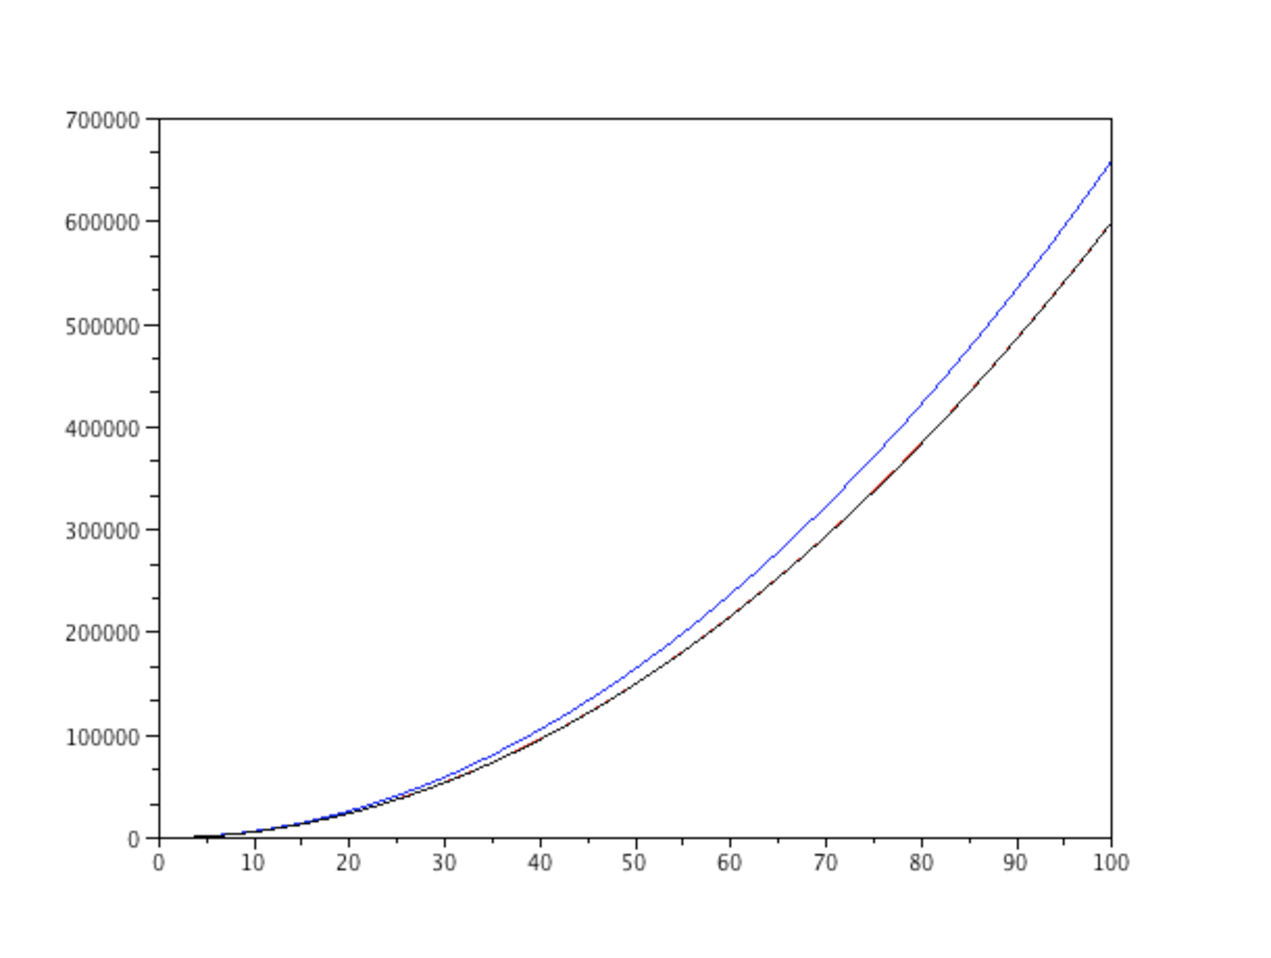
\includegraphics[width=0.7\textwidth]{figuren/telproblemen/01voorbeeld21.png}
\caption{De functie $f(n)=60n^2+5n+1$, zijn ondergrens $f_o(n)=60n^2$ en bovengrens  $f_b(n)=66n^2$. }
\label{fig:vb21}
\end{center}
\end{figure}


\voorbeeld
We zoeken een $\Theta$-notatie voor de functie van de som van de eerste $n$ natuurlijke getallen berekent.
Om een bovengrens te berekenen, gebruiken we dat elk getal uit de som kleiner is dan het grootste getal $n$:
\[
1+2+\dots+n\leq n+n+\ldots+n=n\cdot n=n^2\,.
\]
Hieruit volgt
\[1+2+\dots+n=O(n^2)\]\,.

Om een benedengrens te berekenen gaan we analoog te werk: elke term van de som is groter dan 1:
\[
1+2+\dots+n\geq1+1+\ldots1=n
\]
waaruit we besluiten
\[
1+2+\dots+n=\Omega(n)\,.
\]
\begin{figure}[htbp]
\begin{center}
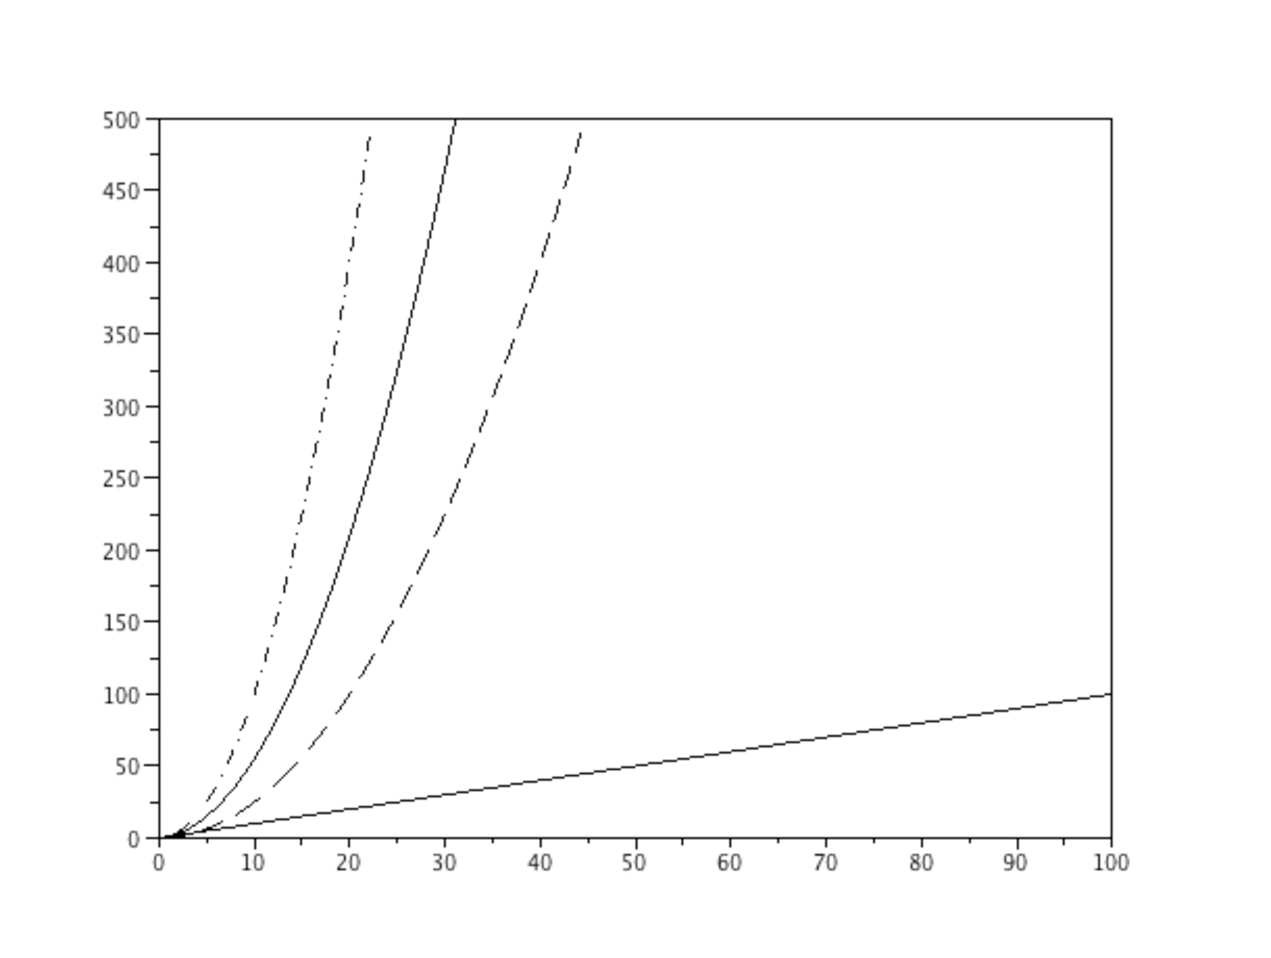
\includegraphics[width=0.7\textwidth]{figuren/telproblemen/03voorbeeld}
\caption{De functie $f(n)=1+\dots n$ (volle lijn bovenaan), de ondergrens $f_{o_1}(n)=n$ (volle lijn onderaan), de ondergrens $f_{o_2}(n)=n^2/4$ (stippellijn) en bovengrens $f_b(n)=n^2$ (punt-streep-lijn)}.
\label{fig:03voorbeeld}
\end{center}
\end{figure}

Op deze manier vinden we geen $\Theta$-notatie want $O$ en $\Omega$ zijn niet van dezelfde orde. Dit komt doordat we de functie te sterk afgeschat hebben. Dit blijkt ook uit figuur~\ref{fig:03voorbeeld}. De af te schatten functie is de volle lijn bovenaan. De bovengrens $n^2$ is de bovenste kromme (streepje-punt-lijn). Deze functie stijgt ongeveer even snel als de oorspronkelijke functie.  Onderaan de figuur zie je de lineaire functie. Het gedrag van deze functie is helemaal anders dan de kwadratische functie. We maken daarom een nieuwe, minder sterke afschatting. Daarbij gaan we als volgt te werk: we laten de eerste helft van de termen weg\footnote{De functie $\text{ceil}(x)$ rondt het getal $x$ naar boven af.}
\begin{eqnarray*}
1+2+\dots+n&\geq& \text{ceil}(n/2)+\ldots+(n-1)+n\\&\geq& n/2+\ldots+n/2+n/2\\
&=&((n+1)/2)(n/2) \\
&\geq& (n/2)(n/2)\\&=&n^2/4
\end{eqnarray*}
Dit geeft de meer nauwkeurige afschatting
\[1+2+\dots+n=\Omega(n^2)
\]
zodat
\[
1+2+\dots+n=\Theta(n^2)\,.
\]
Op figuur~\ref{fig:03voorbeeld} is duidelijk te zien dat de gegeven functie $f(n)=1+\dots n$ omgeven wordt door de functies $f_b(n)=n^2$ en $f_{o_2}(n)=n^2/4$.

\subsection{Uitvoeringstijd}

We spreken over 
\begin{description}
\item[best-case time] minimale hoeveelheid tijd nodig om het programma uit te voeren als de grootte van de input $n$ bedraagt;
\item[worst-case time] maximale hoeveelheid tijd nodig om het programma uit te voeren;
\item[average-case time] gemiddelde hoeveelheid tijd nodig om het programma uit te voeren.
\end{description}

\begin{description}
\item[best-case time] Veronderstel dat een algoritme $t(n)$ tijdseenheden nodig heeft om uitgevoerd te worden. De veranderlijke $n$ is de grootte van de invoer. De functie  $t(n)$ is de minimale uitvoeringstijd: de input is zò gekozen dat het algoritme zo weinig mogelijk stappen nodig heeft om uitgevoerd te worden. Als 
$t(n)=O(g(n))$, dan is de best-case time ten hoogste van orde $g(n)$ en de best-case time is $O(g(n))$.
\item[worst-case time] Veronderstel dat een algoritme $t(n)$ tijdseenheden nodig heeft om uitgevoerd te worden. De veranderlijke $n$ is de grootte van de invoer. De functie $t(n)$ is de maximale uitvoeringstijd: de input is zò gekozen dat het algoritme het maximaal aantal stappen nodig heeft. Als 
$t(n)=O(g(n))$, dan is de worst-case time ten hoogste van orde $g(n)$ en de worst-case time is $O(g(n))$.
\item[average-case time] Veronderstel dat een algoritme $t(n)$ tijdseenheden nodig heeft om uitgevoerd te worden. De veranderlijke $n$ is de grootte van de invoer en de functie $t(n)$ is de gemiddelde uitvoeringstijd. Als $t(n)=O(g(n))$, dan is de average-case time ten hoogste van orde $g(n)$ en de average-case time is $O(g(n))$.

\end{description}

Als hierboven $O$ vervangen wordt door $\Omega$ en ``ten hoogste'' door ``ten minste'', bekomen we de definitie van best-case time, worst-case time en average-case time \emph{ten minste} van orde $g(n)$. 

Als de best-case time van het algoritme $O(g(n))$ is én $\Omega(g(n))$, zeggen we dat de best-case time is $\Theta(g(n))$. De definitie van worst-case time en average-case time is analoog.

\subsection{Voorbeelden}
\voorbeeld

We bekijken als voorbeeld een algoritme om een getal $x$ te zoeken in een rij niet-geordende getallen. Het algoritme geeft de positie van $x$ aan als $x$ voorkomt in de rij. Als $x$ niet voorkomt in de rij, geeft het algoritme het cijfer $0$ als output.

\begin{lstlisting}[caption={Algoritme: zoek getal $x$ in rij $R$}, label={lst:zoek}]
function y=zoek(R,x)
  y=0;
  i=1;
  // zoek x in de rij R
  while (i<=length(R))&(R(i)<>x)
    i=i+1;
  end;
  // als x gevonden is, geef juiste return
  if (i<=length(R))
    y=i;
  end
endfunction
\end{lstlisting}

We nemen het aantal keer dat de vergelijking \lstinline{R(i)==x} uitgevoerd wordt als maat voor de uitvoeringstijd. Het te zoeken getal $x$ kan zich op positie \lstinline{1, ..., n} in de rij bevinden of zich niet in de rij bevinden. Er zijn dus \lstinline{n+1} mogelijke uitkomsten.

\begin{description}
\item[best-case time] Het algoritme is het snelst beëindigd als \lstinline{x} zich op de eerste positie van \lstinline{R} bevindt, dus de best-case time van algoritme~\ref{lst:zoek} is $\Theta(1)$.

\item[worst-case time] De uitvoeringstijd is maximaal als \lstinline{x} zich \emph{niet} in de rij bevindt. Dan moet de test  \lstinline{R(i)==x} \lstinline{n+1} keer uitgevoerd worden. De worst-case time van algoritme~\ref{lst:zoek} is $\Theta(n)$.

\item[average-case time] Om de average-case time te berekenen, tellen we de uitvoeringstijd van alle mogelijkheden (\lstinline{n+1} in totaal) op en delen we die tijd door het aantal mogelijkheden. Als \lstinline{x} gevonden wordt op positie \lstinline{i}, worden er \lstinline{i} vergelijkingen uitgevoerd. Als \lstinline{x} zich niet in de rij bevindt, worden er \lstinline{n} vergelijkingen uitgevoerd. Het gemiddeld aantal keer dat de test uitgevoerd wordt is dus gelijk aan
\[
\frac{(1+2+\dots+n)+n}{n+1}\,.
\]
Analoog met voorgaande voorbeelden berekenen we
\begin{eqnarray*}
\frac{(1+2+\dots+n)+n}{n+1}&\leq& \frac{n^2+n}{n+1}\\
&=& \frac{n(n+1)}{n+1}=n\,.
\end{eqnarray*}
De average-case time van algoritme ~\ref{lst:zoek} is $O(n)$.

Verder hebben we
\begin{eqnarray*}
\frac{(1+2+\dots+n)+n}{n+1}&\geq& \frac{n^2/4+n}{n+1}\\
&\geq& \frac{n^2/4+n/4}{n+1}=\frac n4\,.
\end{eqnarray*}
De average-case time van  algoritme~\ref{lst:zoek} is $\Omega(n)$ zodat de average-case time van algoritme~\ref{lst:zoek} $\Theta(n)$ is.

\end{description}

\voorbeeld

Bepaal een theta notatie in functie van $n$ voor het aantal keer dat de toekenning \lstinline{x=x+1} wordt uitgevoerd in listing~\ref{lst:theta}.

\begin{lstlisting}[caption={Bepaal een theta notatie}, label={lst:theta}]
for i=1:n
  for j=1:i
    x=x+1;
  end
end
\end{lstlisting}

Als $i=1$, neemt $j$ enkel de waarde $1$ aan en wordt de toekenning $x=x+1$ slechts één keer uitgevoerd. Als $i=2$, neemt $j$ de waarden $1$ en $2$ aan en wordt de toekenning twee keer uitgevoerd. Als $i=n$, neemt $j$ de waarden $1,\dots,n$ aan en wordt de toekenning $n$ keer uitgevoerd. In totaal wordt de toekenning dus
\[
1+2+\dots+n=\Theta(n^2)
\]
keer uitgevoerd.

\voorbeeld

Bepaal een theta notatie in functie van $n$ voor het aantal keer dat de toekenning \lstinline{x=x+1} wordt uitgevoerd in listing~\ref{lst:theta2}. Als maat voor de uitvoeringstijd nemen we het aantal keer dat de toekenning $x=x+1$ wordt uitgevoerd. We noteren die met  $t(n)$.
\begin{lstlisting}[caption={Bepaal een theta notatie}, label={lst:theta2}]
j=n;
while (j>=1)
  for i=1:j
    x=x+1;
  end
  j=floor(j/2);
end
\end{lstlisting}

De eerste keer dat de \lstinline{while}-lus uitgevoerd wordt, is $j=n$. De toekenning $x=x+1$ wordt dus minstens $n$ keer uitgevoerd en $t(n)=\Omega(n)$.

Nu zoeken we een bovengrens voor $t(n)$. De eerste keer dat de \lstinline{while}-lus uitgevoerd wordt, is $j=n$ en wordt de toekenning \lstinline{x=x+1} $n$ keer uitgevoerd. In lijn 6 wordt de waarde van $j$ gehalveerd en is $j\leq n/2$. De tweede keer dat de lus uitgevoerd wordt, wordt de toekenning hoogstens $n/2$ keer uitgevoerd. Veronderstel dat $k$ het aantal keer is dat we de \lstinline{while}-lus doorlopen (bereken de waarde van $k$ met behulp van de definitie van de logaritmische functie). Dan is het aantal keer dat de toekenning  \lstinline{x=x+1} uitgevoerd wordt kleiner dan
\[
n+\frac n2+\frac n4+\dots+\frac n{2^{k-1}}\,.
\]
Dit is een som van elementen van een meetkundige rij en gelijk aan
\[
\frac{n\left(1-\frac1{2^k}\right)}{1-\frac12}\,.
\]
Hieruit volgt
\[
t(n)\leq\frac{n\left(1-\frac1{2^k}\right)}{1-\frac12}=2n\left(1-\frac1{2^k}\right)\leq2n
\]
zodat $t(n)=O(n)$. Hieruit bekomen we een $\Theta$-notatie voor het aantal keer dat we de toekenning  $x=x+1$ uitvoeren, namelijk $\Theta(n)$.

\subsection{Oefeningen}
\begin{enumerate}

\item Bepaal de theta notatie van volgende veeltermen. Kies uit $\Theta(1)$, $\Theta(n)$, $\Theta(n^2)$, $\Theta(n^3)$, $\Theta(\log n)$, $\Theta(n\log n)$.
\begin{enumerate}
\item $6n+1$
\item $6n^3+12n^2+1$
\item $2+4+6+\dots+2n$
\item $(6n+4)(1+\log n)$
\end{enumerate}

\item Bepaal een theta notatie voor het aantal keer dat de instructie \lstinline{x=x+1} wordt uitgevoerd.
Kies uit $\Theta(1)$, $\Theta(n)$, $\Theta(n^2)$, $\Theta(n^3)$, $\Theta(\log n)$, $\Theta(n\log n)$.
\begin{lstlisting}[caption={Oefening 2.1}, label={lst:oef21}]
for i=1:2n
  x=x+1
end
\end{lstlisting}
\begin{lstlisting}[caption={Oefening 2.2}, label={lst:oef22}]
for i=1:n
  for j=1:n
    x=x+1
  end
end
\end{lstlisting}
\begin{lstlisting}[caption={Oefening 2.3}, label={lst:oef23}]
for i=1:n
  for j=1:n
    for k=1:i
      x=x+1
    end
  end
end
\end{lstlisting}
\begin{lstlisting}[caption={Oefening 2.4}, label={lst:oef24}]
j=n;
while j>=1
  for i=1:j
    x=x+1;
  end
  j=floor(j/3);
end
\end{lstlisting}
\begin{lstlisting}[caption={Oefening 2.5}, label={lst:oef25}]
i=n;
while i>=1
  for j=1:n
   x=x+1;
 end
  i=floor(i/2);
end

\end{lstlisting}
\end{enumerate}


\vbsection{Telproblemen: Product- en somregel}

In een restaurant kan de klant zijn menu samenstellen uit 2 voorgerechten, 3 hoofdgerechten en 4 dranken. Hoeveel verschillende menu's kan de klant samenstellen uit één hoofdgerecht en één drank? Hoeveel verschillende menu's kan de klant samenstellen uit één voorgerecht, één hoofdgerecht en één drank?

De antwoorden zijn $12=3\cdot 4$ en $24=2\cdot 3\cdot 4$. Dit wordt geïllustreerd in figuur~\ref{fig:hamburgers}.  Het aantal menu's is het product van het aantal voorgerechten, hoofdgerechten en dranken. Dit illustreert de \emph{productregel}.

\begin{figure}[htbp]
\begin{center}
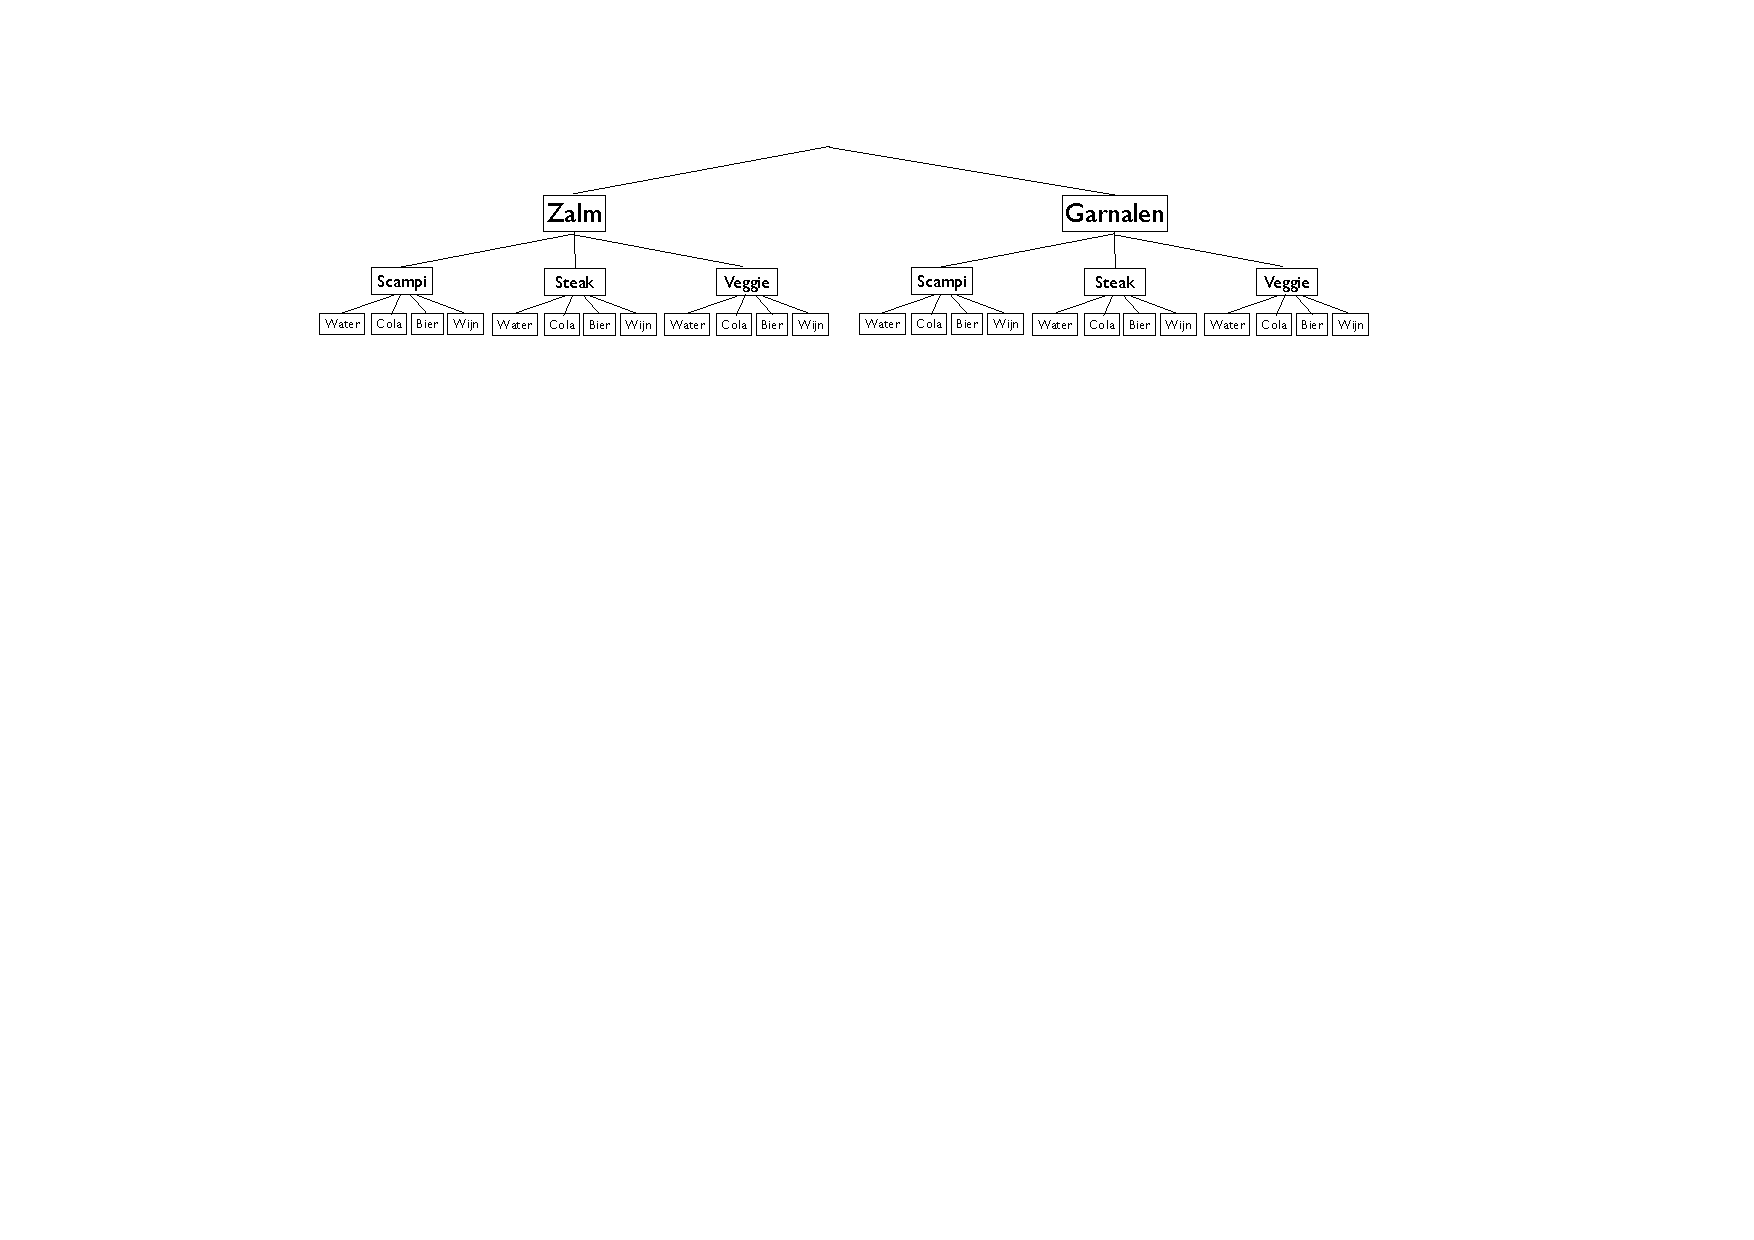
\includegraphics[width=\textwidth]{figuren/telproblemen/04hamburgers}
\caption{Voorbeeld van de productregel.}
\label{fig:hamburgers}
\end{center}
\end{figure}


\subsection{Productregel}
Als een activiteit geconstrueerd kan worden door $t$ opeenvolgende stappen en stap 1 kan gebeuren op $n_1$ manieren, stap 2 op $n_2$ manieren, \dots\ en stap $t$ kan gedaan worden op $n_t$ manieren, dan is het totaal aantal mogelijke activiteiten gelijk aan $n_1\cdot n_2\cdot \dots\cdot n_t$.

\voorbeeld
Hoeveel menu's kunnen er in voorgaand voorbeeld samengesteld worden als de drank niet verplicht is?

Een menu samenstellen zien we als een activiteit die geconstrueerd is door 3 opeenvolgende stappen. Bij stap 1 kiest de klant het voorgerecht. Dat kan op 2 manieren ($n_1=2$). Bij stap 2 kiest de klant het hoofdgerecht. Dat kan op 3 manieren ($n_2=3$). Ten slotte kiest de klant een drank uit de vier mogelijkheden of geen drank. Dat kan op 5 manieren ($n_3=5$). De productregel zegt dan dat de activiteit kan gebeuren op $n_1\cdot n_2\cdot n_3=2\cdot3\cdot5=30$ manieren.

\voorbeeld
\begin{enumerate}
\item Hoeveel strings van lengte 4 kunnen er gevormd worden met de letters {\sc abcde}? Elke letter mag  maar één keer voorkomen.

Gebruik de productregel. Een string wordt geconstrueerd in 4 opeenvolgende stappen. In de eerste stap wordt de eerste letter gekozen. Daarvoor zijn 5 mogelijkheden ($n_1=5$). Dan wordt de tweede, derde en vierde letter gekozen. Daarvoor zijn resp.\  4, 3, en 2 mogelijkheden ($n_2=4$, $n_3=3$, $n_4=2$). De productregel zegt dat er in totaal $n_1\cdot n_2\cdot n_3\cdot n_4=5\cdot4\cdot3\cdot 2=120$ manieren zijn.
\item Hoeveel strings uit voorgaande oefening beginnen met {\sc b}?

Een string die begint met de letter {\sc b} wordt opnieuw geconstrueerd in 4 stappen. Kies de eerste letter (1 mogelijkheid, namelijk {\sc b}). Kies de tweede letter (4 mogelijkheden: alle letters behalve {\sc b}), kies de derde letter (3 mogelijkheden: niet {\sc b} en de letter gekozen in de tweede stap), kies de vierde letter (2 mogelijkheden). Het totaal aantal mogelijkheden is dan gelijk aan $1\cdot 4\cdot 3\cdot 2=24$.
\item Hoeveel strings uit de eerste oefening beginnen niet met de letter {\sc b}?

Het gezochte aantal is gelijk aan het aantal mogelijkheden uit het eerste item minus het aantal mogelijkheden uit het tweede item, dus $120-24=96$.
\end{enumerate}

\voorbeeld
In een bitmap wordt de kleur van elke pixel weergegeven met 8 bit. Hoeveel kleuren zijn er mogelijk per pixel?

De kleur van een pixel is een proces dat bestaat uit 8 opeenvolgende stappen: kies de kleur voor bit 1, kies de kleur voor bit 2 etc. Voor elke bit zijn er twee mogelijkheden. In totaal zijn er dus $2\cdot 2 \cdot 2\cdot \dots\cdot2=2^8=256$ mogelijkheden.

\voorbeeld
Hoeveel kleuren uit voorgaand voorbeeld beginnen met 101 òf 111?

Om een kleur te bepalen die begint met 101, blijven er maar 5 bits over om te kiezen. In totaal zijn er $2^5=32$ kleuren die beginnen met 101. Hetzelfde geldt voor kleuren die beginnen met 111. Om het aantal kleuren te bepalen die beginnen met 101 òf 111, zetten we twee stappen: kies uit 101 en 111 (2 mogelijkheden) en kies dan de string die erna komt (32 mogelijkheden). Het antwoord voor bovenstaande vraag is dus $2\cdot 32=64$ of $32+32$.

\subsection{Somregel}
In voorbeeld~\thesection.\arabic{vb} telden we het aantal kleuren van ieder soort op. De \emph{somregel} leert ons wanneer we moeten optellen om het totaal aantal mogelijkheden te bekomen.

Veronderstel dat $X_1,~X_2,~\dots,~X_t$ verzamelingen zijn en dat de $i$-de verzameling $n_i$ elementen bevat. Als de verzamelingen $X_1,~X_2,~\dots,~X_t$  twee aan twee geen gelijke elementen bevatten (d.w.z., als $i\neq j$, $X_i\cap X_j=\emptyset$), dan is het aantal van mogelijke elementen die uit $X_1$ of $X_2$ of \dots\ of $X_t$ komen, gelijk aan \[n_1+n_2+\dots+n_t\,.\]
In andere woorden: het aantal elementen van iedere deelverzameling moet opgeteld worden als de deelverzamelingen twee aan twee geen elementen gemeen hebben.

\voorbeeld
Op een boekenplank staan 5 verschillende boeken over computers, drie verschillende boeken over wiskunde en twee verschillende kunstboeken. Op hoeveel manieren kan je twee boeken kiezen met verschillend onderwerp?

Je kan op $5\cdot 3=15$ manieren een computer- met een wiskundeboek combineren. Noem de verzameling van die duo's $X_1$. Je kan op $5\cdot2=10$ manieren een computer- met een kunstboek combineren (verzameling $X_2$). Ten slotte kan je op $3\cdot 2=6$ manieren een wiskunde- met een kunstboek combineren ($X_3$). Uit de verzamelingen $X_1$, $X_2$ en $X_3$ moet je uiteindelijk een duo boeken kiezen. De elementen van die verzameling zijn allemaal verschillend. De somregel zegt dan dat je keuze hebt uit de som van het aantal elementen van die verzamelingen $15+10+6=31$.

\voorbeeld
Alien, Bob, Chris, David, Erik en Frances vormen een club. Ze kiezen een voorzitter, penningmeester en secretaris. De jobs kunnen niet gecombineerd worden.
\begin{enumerate}
\item Op hoeveel verschillende manieren kunnen ze die jobs verdelen?

De keuze is een activiteit die bestaat uit 3 verschillende stappen. De productregel zegt dat er $6\cdot5\cdot 4=120$ mogelijkheden zijn.
\item Op hoeveel verschillende manieren kunnen ze die jobs verdelen als ofwel Bob ofwel Alien voorzitter moet zijn?

De activiteit bestaat uit 3 stappen. Voor de keuze van de voorzitter zijn er 2 mogelijkheden. Voor de keuze van de penningmeester en secretaris zijn er resp.\ 5 en 4 mogelijkheden. Het totaal aantal manieren is dus gelijk aan $2\cdot 5\cdot 4=40$.
\item Hoeveel mogelijkheden zijn er als Erik zeker één taak op zich neemt?

Stap 1: Erik kiest een taak (3 mogelijkheden). Stap 2: Uit de 5 anderen wordt iemand gekozen voor de tweede taak. Stap 3:  Uit de 4 anderen wordt iemand gekozen voor de derde taak.  Het totaal aantal mogelijkheden is dus $3\cdot5\cdot4=60$.
\item Hoeveel mogelijkheden zijn er als David en Frances allebei een taak op zich nemen?

Stap 1: David kiest een taak (3 mogelijkheden). Stap 2: Frances kiest een taak (2 mogelijkheden). Stap 3: de overblijvende taak wordt toegekend aan één van de overblijvers (4 mogelijkheden). Er zijn dus in totaal $3\cdot2\cdot4=24$ mogelijkheden.
\end{enumerate}

\subsection{Oefeningen}
\begin{enumerate}
\item Er wordt een rode en een blauwe dobbelsteen geworpen.
\begin{enumerate}
\item Hoeveel verschillende worpen zijn er?
\item Voor hoeveel verschillende worpen is de som gelijk aan 4?
\item Bij hoeveel worpen hebben beide dobbelstenen evenveel ogen?
\item Bij hoeveel worpen is de som gelijk aan 7 òf aan 11?
\item Bij hoeveel worpen heeft de blauwe dobbelsteen 2 ogen?
\item Bij hoeveel worpen is er juist één dobbelsteen met 2 ogen?
\item Bij hoeveel worpen heeft minstens één dobbelsteen 2 ogen?
\item Bij hoeveel worpen heeft geen enkele dobbelsteen 2 ogen?
\item Bij hoeveel worpen is de som van beide ogen een even getal?
\end{enumerate}

\item We nemen de getallen 5 tot en met 200.
\begin{enumerate}
\item Hoeveel getallen zijn er?
\item Hoeveel getallen zijn even?
\item Hoeveel getallen zijn oneven?
\item Hoeveel getallen zijn deelbaar door 5?
\item Hoeveel getallen zijn strikt groter dan 72?
\item Hoeveel getallen zijn samengesteld uit verschillende cijfers?
\item Hoeveel getallen zijn samengesteld uit twee verschillende cijfers?
\item Hoeveel getallen bevatten het cijfer 0?
\item Hoeveel getallen bevatten niet het cijfer 0?
\item Hoeveel getallen zijn groter dan 101 én bevatten niet het cijfer 6?
\item Hoeveel getallen zijn samengesteld uit cijfers die steeds groter zijn (bijvoorbeeld 13, 147, 8)?
\item Hoeveel getallen zijn van de vorm $xyz$ waarbij $0\neq x< y$ en $y>z$?
\end{enumerate}


\end{enumerate}
\vbsection{Telproblemen: Permutaties, variaties en combinaties}

\subsection{Permutaties}
De geordende rij $x_1,~x_2,\dots,~x_n$ van $n$ verschillende elementen is de \emph{permutatie} van  $x_1,~x_2,\dots,~x_n$.
Er zijn $n!$ permutaties van $n$ elementen.

\voorbeeld
Er zijn 6 permutaties van 3 elementen $A$, $B$ en $C$: $ABC$, $ACB$, $BAC$, $BCA$, $CAB$ en $CBA$.

\voorbeeld
Hoeveel permutaties van de letters $ABCDEF$ bevatten de substring $DEF$? 

Dit is een permutatie van 4 elementen namelijk $A$, $B$ en $C$ en de string $DEF$. Dat geeft $4!=24$ permutaties.

\voorbeeld 
Hoeveel permutaties van de letters $ABCDEF$ bevatten de letters $D$, $E$ en $F$ opeenvolgend in eender welke volgorde?

We lossen dit probleem op in 2 stappen. Stap 1: maak een permutatie van de letters $D$, $E$ en $F$. Hiervoor zijn $3!=6$ mogelijkheden. Stap 2: maak een permutatie met de letters $A$, $B$, $C$ en de permutatie van stap 1. Hiervoor zijn $4!=24$ mogelijkheden. Gebruik de productregel om het antwoord op de vraag te bekomen: $6\cdot 24=144$.

\voorbeeld
Op hoeveel verschillende manieren kunnen 6 personen rond een ronde tafel gaan zitten? Als alle personen één plaats opschuiven, wordt dat niet als een nieuwe situatie beschouwd.

Noem de personen $A$, $B$, \dots, $F$. Omdat rotaties niet meegerekend worden, geven we persoon $A$ alvast een plaats. Er vallen dan nog 5 personen te verdelen over 5 plaatsen. Daarvoor zijn $5!=120$ mogelijkheden.

\subsection{Variatie van $r$ elementen uit $n$}
Een variatie van $r$ elementen uit $n$ verschillende elementen $x_1,~x_2,\dots,~x_n$ is een geordende deelverzameling van $r$ elementen uit $\{x_1,~x_2,\dots,~x_n\}$. 
We noteren $V(n,r)$. Het aantal variaties van $r$ elementen uit $n$ elementen is gelijk aan \[V(n,r)=\frac{n!}{(n-r)!}=n(n-1)(n-2)\dots(n-r+1)\quad r\leq n\,.\]

\voorbeeld
De variaties van 2 elementen uit $X=\{a,b,c\}$ zijn $ab$, $ac$, $ba$, $bc$, $ca$, $cb$.

\voorbeeld
Op hoeveel verschillende manieren kunnen er een voorzitter, ondervoorzitter, penningmeester en secretaris gekozen worden uit een groep van 10 personen?

Uit de groep van 10 personen moet een geordende rij van 4 personen gekozen worden (de plaats in de rij bepaalt de functie). Dit is een variatie van 4 elementen uit 10. Het aantal mogelijkheden is gelijk aan 
\[
V(10,4)=\frac{10!}{6!}=10\cdot9\cdot8\cdot7=5040
\]

\subsection{Combinaties}
Gegeven de verzameling $\{x_1,~x_2,\dots,~x_n\}$ van $n$ verschillende elementen.
\begin{itemize}
\item De combinatie van $r$ elementen uit $n$ van $X$ is de niet-geordende verzameling van $r$ elementen uit $X$.
\item Het aantal combinaties van $r$ elementen uit $n$ is gelijk aan \[C(n,r)={n \choose r}=\frac {V(n,r)}{r!}\]
\end{itemize}

\voorbeeld
Op hoeveel verschillende manieren kan je 3 mensen kiezen uit een groep van 10 verschillende mensen?

De volgorde waarop de mensen gekozen zijn is niet belangrijk. Het aantal manieren bedraagt dus
\[
C(10,3)=\frac{V(10,3)}{3!}=\frac{10!}{7!\cdot3!}=120
\]

\voorbeeld
Op hoeveel manieren kan je twee vrouwen en drie mannen kiezen uit een groep bestaande uit vijf vrouwen en zes mannen?

Je kan de vrouwen kiezen op $C(5,2)=10$ manieren. De mannen kan je kiezen op $C(6,3)=20$ manieren. De productregel geeft dat je de totale keuze kan maken op $10\cdot 20=200$ manieren.

\voorbeeld
Hoeveel strings van 8 bit bevatten juist vier enen?

Om dit aantal te tellen, moet je nagaan op hoeveel manieren je de vier enen kan plaatsen. Daarvoor moet je 4 posities kiezen uit 8 mogelijkheden, wat dus neerkomt op $C(8,4)=70$.

\subsection{Oefeningen}

\begin{enumerate}
\item Hoeveel permutaties zijn er van $a$, $b$, $c$ en $d$?
\item Noteer alle permutaties van $a$, $b$, $c$ en $d$.
\item Hoeveel variaties van 3 elementen zijn er uit $a$, $b$, $c$ en $d$?
\item Noteer alle variaties van 3 elementen uit $a$, $b$, $c$ en $d$.
\item Hoeveel permutaties zijn er van 11 verschillende elementen?
\item Hoeveel variaties van 5 elementen zijn er uit 11 verschillende elementen?
\item Hoeveel combinaties van 3 elementen zijn er uit $X=\{a,b,c,d\}$?
Noteer deze combinaties.
\item Een club telt 6 verschillende mannen en 7 verschillende vrouwen.
\begin{enumerate}
\item Op hoeveel manieren kunnen we een staf selecteren van 5 personen?
\item Op hoeveel manieren kunnen we een staf samenstellen die bestaat uit drie mannen en vier vrouwen?
\item Op hoeveel manieren kunnen we een staf samenstellen die bestaat uit 5 personen waarvan er minstens één vrouw is?
\item Op hoeveel manieren kunnen we een staf samenstellen die bestaat uit 5 personen waarvan er minstens één man is?
\item Op hoeveel manieren kunnen we een staf samenstellen die bestaat uit 5 personen zodat elk geslacht vertegenwoordigd is?
\item  Op hoeveel manieren kunnen we een staf samenstellen die bestaat uit 5 personen zodat Martha en Raf niet samen in de staf zitten?
\end{enumerate}
\item Een muntstuk wordt 10 maal opgeworpen.
\begin{enumerate}
\item Hoeveel uitkomsten zijn er? De volgorde van de worpen is van tel!
 \item Hoeveel uitkomsten tellen juist drie keer kop?
 \item Hoeveel uitkomsten tellen minstens drie keer kop?
 \item Hoeveel uitkomsten hebben kop bij de vijfde worp?
 \item Hoeveel uitkomsten tellen evenveel keer kop als munt?
\end{enumerate}

\end{enumerate}


\vbsection{Algoritmes om combinaties en permutaties te genereren}
\subsection{Inleiding}
Een popgroep neemt een aantal songs op met verschillende tijdsduur. Ze hebben plannen om een CD uit te geven. Ze zoeken nu naar de combinatie van songs die én op de CD past én zoveel mogelijk muziek oplevert.

In principe kan dit probleem opgelost worden door alle combinaties van songs uit te proberen en dan die combinatie te weerhouden die aan de voorwaarden voldoet. Er zijn in totaal $2^n$ mogelijke combinaties, zodat de uitvoeringstijd van het bijbehorende algoritme $\Omega(2^n)$ bedraagt. De uitvoeringstijd van dit algoritme wordt bijgevolg snel erg groot als $n$ groter wordt. Jammer genoeg bestaat er voor bovenstaand probleem geen andere oplossing dan `alle mogelijkheden uitproberen'. 

In deze sectie bekijken we algoritmes die zo efficiënt mogelijk alle mogelijke combinaties (en permutaties) genereren.

\subsection{Lexicografische orde}
Een woordenboek is alfabetisch geordend: `woord' komt voor `woordenboek' en `lamp' komt voor `lomp'.  Lexicografische orde is de veralgemening van alfabetische orde: de letters worden vervangen door een geordende verzameling symbolen, bijvoorbeeld de cijfers 0-9. We hebben volgende definitie:

Gegeven zijn twee woorden. We gaan als volgt te werk om te bepalen welk van de twee woorden lexicografisch eerst komt. Er zijn twee mogelijkheden.
\begin{enumerate}
\item De twee woorden hebben verschillende lengte en het lange woord is een verderzetting van het korte woord.
\item De woorden hebben verschillende lengte en het lange woord is \emph{geen} verderzetting van het korte woord.
\item De woorden hebben dezelfde lengte (maar zijn verschillend).
\end{enumerate}
In geval 1 komt het korte woord lexicografisch voor het lange woord (`woord' komt voor `woordenboek'). In geval 2 en 3 zoeken we, te beginnen van links, de eerste letter van beide woorden die verschillend is. De lexicografische volgorde van beide woorden wordt bepaald door de volgorde van die ene letter. Zo komt het woord `raadsel' voor het woord `raamfolie'. De vierde letter is de eerste letter van links te beginnen in beide woorden die verschillend is. De letter `d' komt voor de letter `m'.


\voorbeeld
Als de verzameling symbolen de cijfers $\{1,2,3,4\}$ is, dan komt 
\begin{itemize}
\item $132$ voor $1324$ want het tweede `woord' is langer dan het eerste en verderzetting daarvan (geval 1);
\item $1311$ voor $132$: de twee woorden hebben verschillende lengte. Het derde cijfer is het eerste cijfer van links te beginnen dat verschillend is. Het cijfer $1$ komt voor het cijfer $2$, dus $1311$ komt lexicografisch voor het getal $132$ (geval 2).
\item $1324$ voor $1423$: beide woorden hebben dezelfde lengte. Het tweede cijfer van links te beginnen is verschillend en $3$ komt voor $4$ (geval 3);
\end{itemize}

Merk op dat in voorbeeld~\thesection.\arabic{vb} de lexicografische orde anders is dan de numerieke orde. In hetgeen volgt ordenen we steeds lexicografisch. 

\subsection{Algoritme om combinaties te genereren}
In het algoritme om combinaties te genereren zoeken we alle combinaties van $r$ elementen uit de verzameling $\{1,2,\dots,n\}$. Deze combinaties van $r$ elementen noteren we als de string $s_1~s_2~\dots~s_r$ waarbij $s_1<s_2<\dots<s_r$. Bijvoorbeeld: de combinatie van 3 elementen $\{6,2,4\}$ noteren we met $246$.

De combinaties worden in lexicografische orde gegenereerd, dus eerst de string $12\dots\ r$ en laatst de string $(n-r+1)\dots\ n$.

\voorbeeld
We zoeken de combinaties van 5 elementen uit $\{1,2,3,4,5,6,7\}$. De eerste string is $12345$, gevolgd door $12346$ en $12347$,  $12356$ en $12357$. De laatste string is $34567$.

\voorbeeld
Vind de string die volgt op $13467$ als we de combinaties van 5 elementen uit $\{1,2,3,4,5,6,7\}$ zoeken.

Het derde element van rechts te beginnen (4) is het eerste element van rechts te beginnen dat zijn maximale waarde nog niet bereikt heeft. Dat element wordt opgehoogd tot 5. De elementen die rechts ervan liggen krijgen opeenvolgende waarden. De string die volgt op $13467$ is dus $13567$.

\voorbeeld
Vind de string die volgt op $2367$ als we de combinaties van 4 elementen uit $\{1,2,3,4,5,6,7\}$ zoeken.

Opnieuw is het derde element, van rechts te beginnen, het eerste dat niet zijn maximale waarde bereikt heeft. De string die volgt op $2367$ is dus $2456$.


We merken het volgende. Gegeven de string $s_1~s_2~\dots~s_r$. Om de volgende string $t_1~t_2~\dots~t_r$ te vinden, zoeken we het meest rechtse element $s_m$ dat nog niet zijn maximale waarde heeft ($s_r$ kan maximaal gelijk zijn aan $n$, $s_{r-1}$ heeft als maximale waarde $n-1$ enz.). Dan is
\[
t_i=s_i \quad \mathrm{voor} \quad i=1,\dots, m-1\,.
\]
Het element $t_m$ is gelijk aan $s_m+1$. De overige elementen van de nieuwe string zijn gelijk aan
\[
t_{m+1}=s_m+2,~t_{m+2}=s_m+3,~\dots\ 
\]\\

We bekomen volgend algoritme om combinaties van $r$ elementen uit $n$ te genereren:

\begin{lstlisting}[caption={Algoritme om alle combinaties van $r$ elementen uit $n$ elementen te genereren}, label={lst:alg_comb}]
function y=C(n,r)
    //aantal combinaties van r elementen te kiezen uit n
  y=factorial(n)/(factorial(r)*factorial(n-r))
endfunction

function combinatie(n,r)
  //S is vector met de r getallen
  S=1:r;
  disp(S);  // print de eerste combinatie
  for i=2:C(n,r)
    m=r;
    max_val=n;
    while S(m)==max_val
      // vind het meest rechtse element dat nog niet 
      // zijn maximale waarde heeft bereikt
      m=m-1;
      max_val=max_val-1;
    end
    // hoog dat element op
    S(m)=S(m)+1;
    // de elementen meer naar rechts zijn opeenvolgende cijfers
    for j=m+1:r
      S(j)=S(j-1)+1;
    end
    disp(S)
  end
endfunction
\end{lstlisting}

\subsection{Algoritme om permutaties te genereren}
Ook in het algoritme om permutaties te genereren houden we de lexicografische orde aan.

\voorbeeld
We construeren de permutaties van $\{1,2,3,4,5,6\}$. Welke permutatie volgt lexicografisch op $163542$?\\

Kan de permutatie die volgt op $163542$ beginnen met $1635$? De enige permutatie die mogelijk is, is $163524$, maar die is lexicografisch kleiner dan $163542$, dus dat kan niet.

Kan de permutatie die volgt op $163542$ beginnen met $163$? De laatste drie cijfers moeten een permutatie van $\{2,4,5\}$ zijn. Van die permutaties is $542$ de grootst mogelijke permutatie, dus een permutatie die begint met  $163$ en volgt op $163542$ bestaat niet.

De reden dat de permutatie die volgt op $163542$ niet kan beginnen met $163$ of $1635$ is dat de resterende cijfers $542$ resp.\ $42$ in \emph{dalende} volgorde staan. We moeten dus, van rechts te beginnen,  het eerste cijfer $d$ dat kleiner is dan zijn rechterbuur $r$ zoeken. Hier is dat het derde cijfer (3). Dit derde cijfer is bijgevolg het eerste dat aangepast kan worden. De permutatie die volgt op $163542$ moet dus beginnen met $16$.

Het cijfer dat komt na $16$ moet juist groter zijn dan $3$ en is dus gelijk aan $4$. De overige cijfers moeten van klein naar groot geordend worden en zijn dus gelijk aan $235$.\\

Algemeen hebben we het volgende. Om alle permutaties van $\{1,2,\dots,n\}$ te genereren, beginnen we met de permutatie $12\dots\ n$. We gebruiken de methode zoals beschreven in voorbeeld~\thesection.\arabic{vb} om de volgende permutatie te genereren. De laatste permutatie is $n(n-1)\dots\ 21$. 

Listing~\ref{lst:permutatie} toont een algoritme om alle permutaties van $r$ elementen te genereren.

\begin{lstlisting}[caption={Algoritme om alle permutaties van $r$ elementen te genereren}, label={lst:permutatie}]
function W=wissel(V,x,y)
  // wissel in vector s element x en y van plaats
  W=V;
  W(y)=V(x);
  W(x)=V(y);
endfunction

function permutatie(n)
  // vind alle permutaties van 1...n 
  // in lexicografische volgorde
  V=1:n;
  disp(V);
  for i=2:factorial(n)
    m=n-1;
    while V(m)>V(m+1)
      // zoek het eerste element dat kleiner is dan het
      // tweede te beginnen van rechts
      m=m-1;
    end
    k=n;
    while V(m)>V(k)
      //  vind het meest rechtse element s(k)
      // waarbij s(m)<s(k)
      k=k-1;
    end
    V=wissel(V,m,k);
    p=m+1;
    q=n;
    while p<q
      V=wissel(V,q,p);
      p=p+1;
      q=q-1;
    end
    disp(V)
  end
endfunction
\end{lstlisting}

\subsection{Oefeningen}
\begin{enumerate}
\item Gebruik het algoritme van listing~\ref{lst:alg_comb} om te bepalen welke combinatie van r getallen uit de verzameling $\{1,2,3,4,5,6,7\}$ volgt op
\begin{enumerate}
\item  23467
\item 1356
\item 12367
\item 14567
\end{enumerate}
\item Gebruik het algoritme van listing~\ref{lst:alg_comb} om alle combinaties van 4 elementen uit de verzameling $\{1,2,3,4,5,6\}$ te genereren.
\item Gegeven volgende permutatie van $r$ getallen. Gebruik het algoritme van listing~\ref{lst:permutatie} om te bepalen welke permutatie van $r$ getallen uit de verzameling $\{1,2,3,4,\dots,r\}$ volgt op de gegeven permutatie
\begin{enumerate}
\item 12354 ($r=5$)
\item 625431 ($r=6$)
\item 12876543 ($r=8$)
\end{enumerate}
\item Gebruik het algoritme van listing~\ref{lst:permutatie} om alle permutaties uit de verzameling $\{1,2,3,4\}$ te bepalen.
\end{enumerate}


